\section{L'usine logicielle de
Vitameal}\label{lusine-logicielle-de-vitameal}

L'usine logicielle de Vitameal répond aux exigences suivantes :

\begin{itemize}
\tightlist
\item
  respecter les régles de qualitées ;
\item
  avoir une documentation claire et intégrée au projet ;
\item
  gerer les erreurs et assurer leurs suivies ;
\item
  versionnionner le code source et la documentation ;
\item
  avoir un espace commun accessible à distance ;
\item
  gérer un espace de livraison génerant des indicateurs de santé sur le
  projet ;
\item
  avoir un outil de conception UML couvrant la methode minimal UML ;
\item
  gérer la planification du projet.
\end{itemize}

\subsection{Outils utilisés}\label{outils-utilisuxe9s}

Les outils utilisées par l'usine logicielle de Vitameal se sépare en
deux catégories :

\begin{itemize}
\tightlist
\item
  Le côté poste de développement qui correspond aux outils installés par
  chaque développeur sur sa machine ;
\item
  Le côté espace d'integration continue qui correspond aux outils
  composant l'espace communs de collaborations.
\end{itemize}

La documentation du projet est assuré par l'utilisation de la syntaxe
\emph{markdown} integré à l'outil \emph{GitHub} et le language de
génération des livrables est \emph{LaTex}.

Le language cible de cette usine est Java, mais elle peut facilement
être adapté à d'autre language.

\subsubsection{Côté poste de
développement}\label{cuxf4tuxe9-poste-de-duxe9veloppement}

\begin{itemize}
\tightlist
\item
  \textbf{Eclipse} comme IDE pour écrire/éditer le code de l'application
  ;
\item
  \textbf{Maven} comme constructeur du projet (gestion des dépendances,
  automatisation de la construction
\item
  \textbf{JUnit} pour ecrire les tests unitaires de l'application et
  \textbf{Codertura} pour analyser la couverture du projet par ces tests
  ;
\item
  \textbf{Git} pour versionner les sources du projet ;
\item
  \textbf{StarUML} pour modéliser selon le standart UML le projet ;
\item
  \textbf{GanttProject} pour plannifier le projet avec un diagramme de
  Gantt ;
\item
  \textbf{TEXMaker} pour éditer les fichiers\texttt{.tex} avec un
  comportement proche des \emph{WYSIWYG} (optionnel).
\end{itemize}

\subsubsection{Côté espace d'integration
continue}\label{cuxf4tuxe9-espace-dintegration-continue}

\begin{itemize}
\tightlist
\item
  \textbf{GitHub} comme gestionnaire à distance du repositorie Git
  principal, comme tracker de bug et comme affichage visuel des taches à
  faire ;
\item
  \textbf{Jenkins} comme serveur d'intégration continue ;
\item
  \textbf{SonarQube} comme analyseur de qualité du code.
\end{itemize}

\subsection{Schema de fonctionnement}\label{schema-de-fonctionnement}

\begin{figure}
\centering
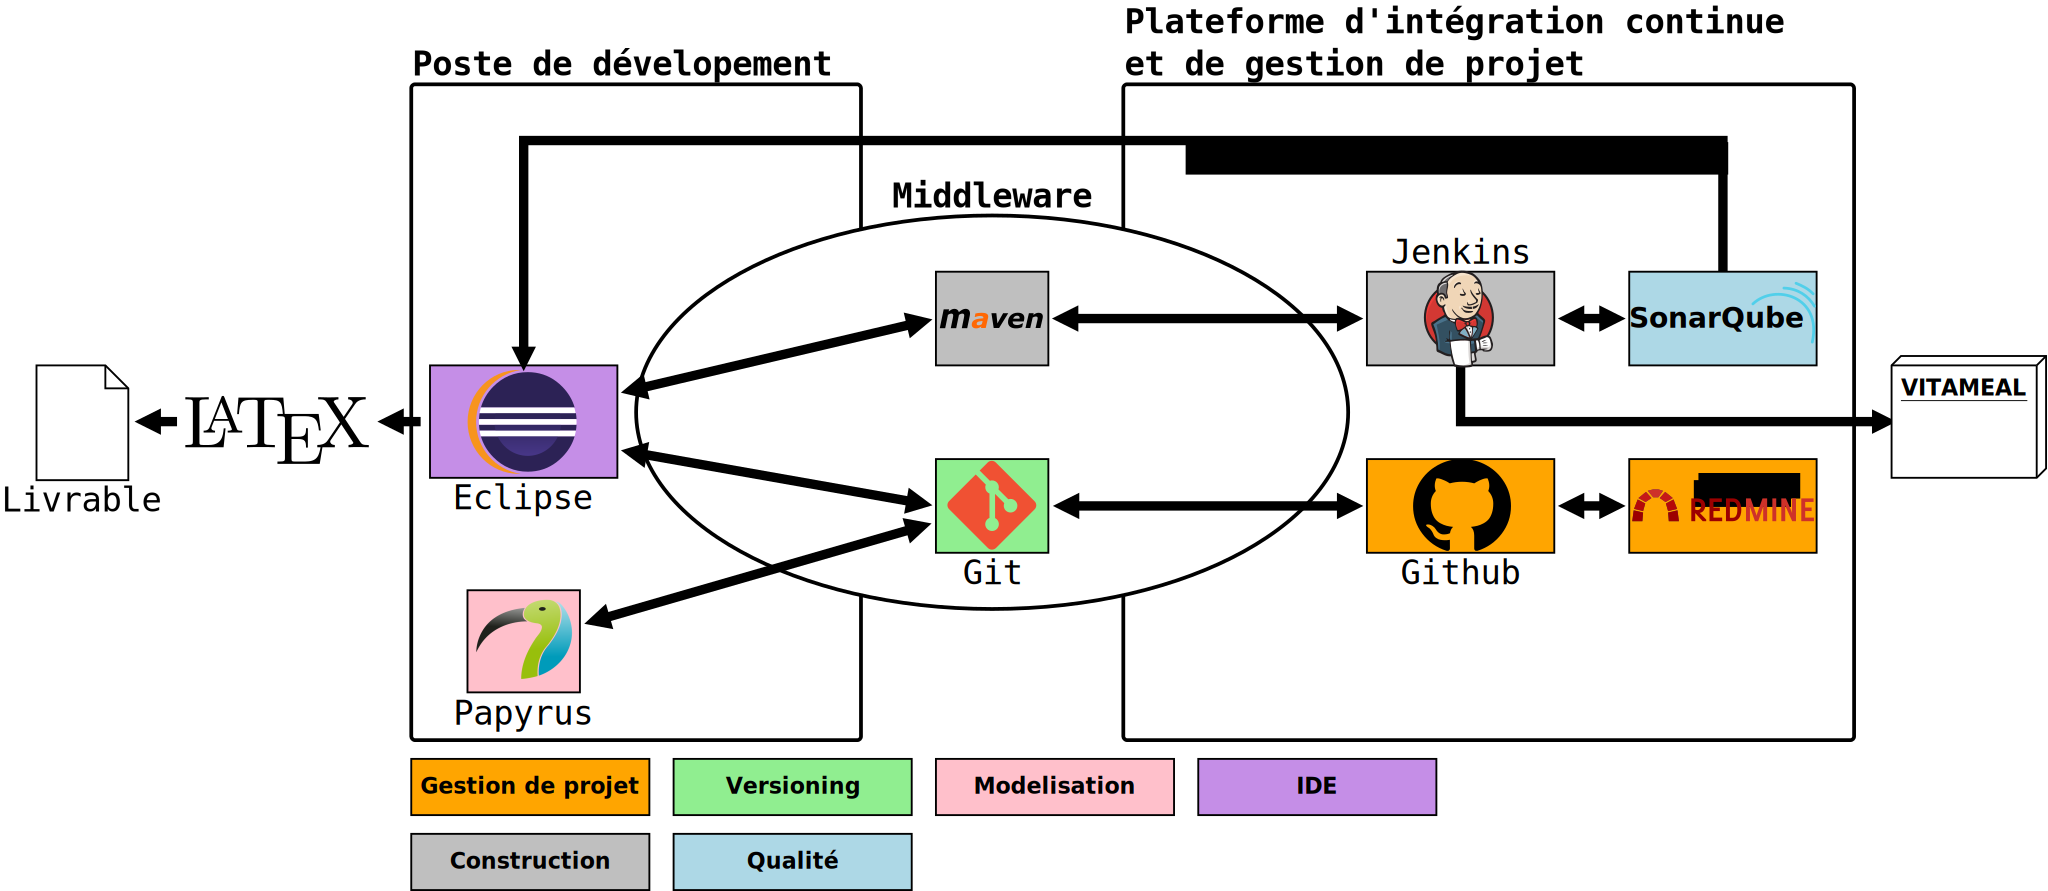
\includegraphics{https://seikomi.github.io/Vitameal/doc/outils/usine_vitameal.svg}
\caption{Usine logicielle de Vitameal}
\end{figure}

\subsection{Installation des outils du poste
développeur}\label{installation-des-outils-du-poste-duxe9veloppeur}

\texttt{TODO}
